\section{Definition and Comparison to Stream Ciphers}

In symmetric cryptography, block ciphers and stream ciphers are two main types.

Stream ciphers encrypt data one bit or one byte at a time. 
They use a \textit{keystream}, where each keystream bit is added to a plaintext bit individually.

\begin{figure}[h] % 'h' means place the figure here if possible
    \centering
    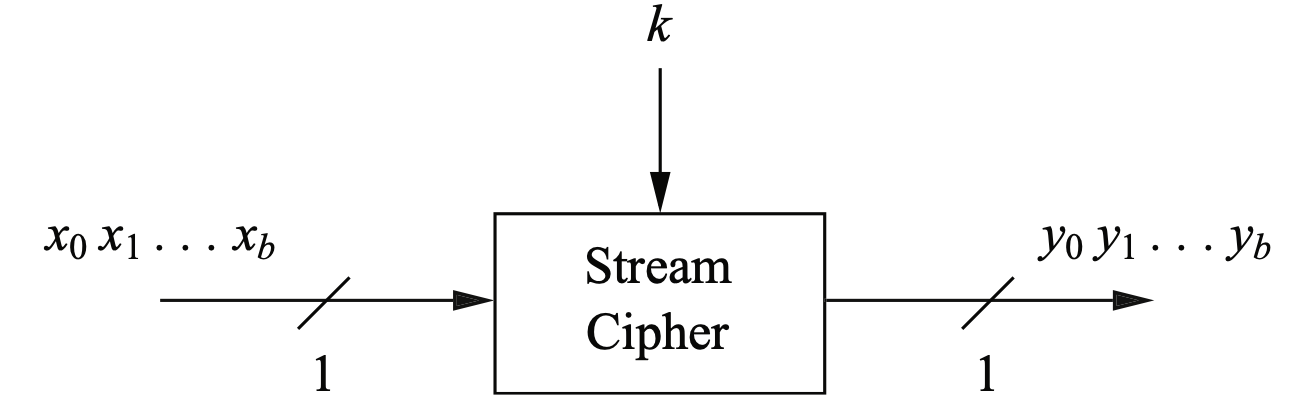
\includegraphics[width=.7\textwidth]{streamc.png}
    \caption{Stream cipher operation}
    \label{fig:stream_cipher}
\end{figure}

Block ciphers process fixed-size blocks of data, with each block encrypted separately.

\begin{figure}[h]
    \centering
    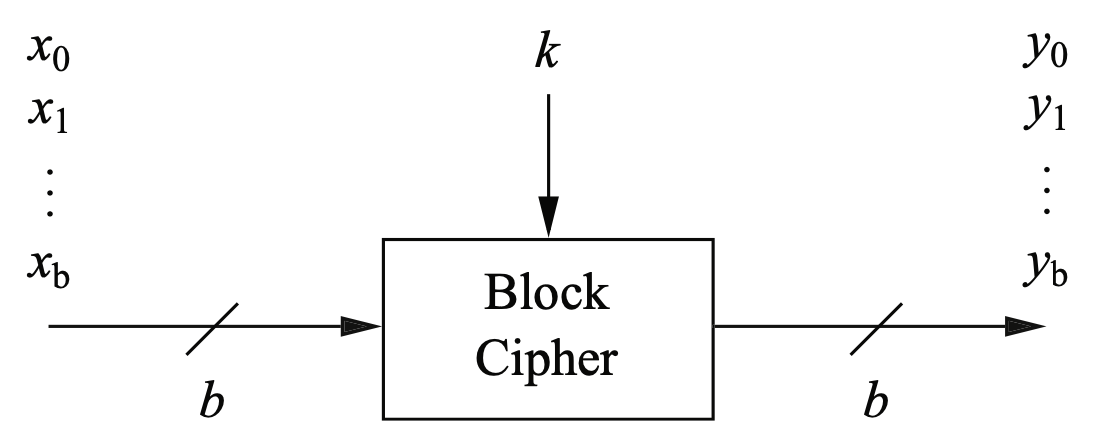
\includegraphics[width=0.7\textwidth]{blockc.png}
    \caption{Block cipher operation}
    \label{fig:block_cipher}
\end{figure}



\begin{table}[h]
\centering
\begin{tabular}{|c|c|}
\hline
\textbf{Block Cipher} & \textbf{Stream Cipher} \\
\hline
Encrypts chunks (blocks) & Encrypts continuously, bit by bit \\
\hline
Offers more security when used properly & Can be faster and have less delay \\
\hline
\end{tabular}
\caption{Comparison between block cipher and stream cipher.}
\label{tab:block_vs_stream}
\end{table}